\documentclass[11pt,twoside]{article}

\usepackage{amsmath}
\usepackage{graphicx,epsfig}
\usepackage{graphicx}
\usepackage{amsmath,amssymb,amsbsy,bm}
%\usepackage[framed]{mcode}

\newlength{\toppush}
\setlength{\toppush}{2\headheight}
\addtolength{\toppush}{\headsep}

\renewcommand{\bottomfraction}{0.95}

\newcommand{\htitle}[3]{\begin{center}
\vspace*{-\toppush}
{\large MASSACHUSETTS INSTITUTE OF TECHNOLOGY}\\
{\small Department of Electrical Engineering and Computer Science}\\
\vspace*{1ex}{\Large #2}\end{center}
\noindent
\newline\parbox{6.5in}
{Fall 2013\hfill Issued : #1 \newline
 Problem Set 1 \hfill Due : #3\newline
%\profs \hfill %Handout #1\vspace*{-.5ex}\newline
%\mbox{}\hrulefill\mbox{}
}}

\newcommand{\mcO}{\mathcal{O}}
\newcommand{\handout}[3]{\thispagestyle{empty}
\pagestyle{myheadings}\htitle{#1}{#2}{#3}}

\setlength{\oddsidemargin}{0pt}
\setlength{\evensidemargin}{0pt}
\setlength{\textwidth}{6.5in}
\setlength{\topmargin}{0in}
\setlength{\textheight}{8.5in}


\newcommand{\pp}[2]{\frac{\partial #1}{\partial #2}}%
\newcommand{\ppp}[2]{\frac{\partial^2 #1}{\partial #2^2}}%
\newcommand{\dd}[2]{\frac{d #1}{d #2}}%
\newcommand{\ddd}[2]{\frac{d^2 #1}{d #2^2}}%
\newcommand{\matend}{\end{array}\right]}
\newcommand{\matc}{\left[\begin{array}{c}}
\newcommand{\matcc}{\left[\begin{array}{cc}}
\newcommand{\bb}{\mathbf{b}}
\newcommand{\bx}{\mathbf{x}}
\newcommand{\bA}{\mathbf{A}}
\newcommand{\DD}[2]{\frac{D #1}{D #2}}%
\newcommand{\Uvec}{\mathbf{U}}
\newcommand{\uvec}{\mathbf{u}}
\newcommand{\tauvec}{\bm{\tau}}
\newcommand{\omegavec}{\bm{\omega}}


\renewcommand{\Re}{\mathrm{Re}}


\begin{document}


\handout{Sept 5, 2013}{6.301 Solid State Circuits}{Sept 12, 2013}
\setlength{\parindent}{0pt}

\newcommand{\solution}{
 \medskip
 {\bf Solution:}
}

\hrulefill

\flushleft

\subsection*{Problem 1: Basic Techniques}
\begin{enumerate}
	\item[(a)] For the following circuit, sketch the pole-zero plot, Bode plot, 
			  and unit step response for $\dfrac{V_2}{V_1}(s)$ and $\dfrac{V_3}{V_1}(s)$.  
\begin{center}
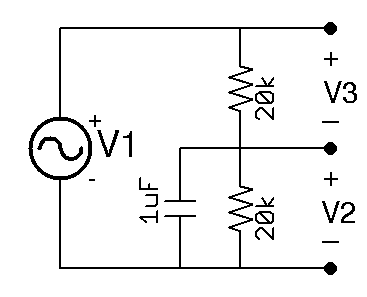
\includegraphics[width=0.3\textwidth]{tf.png}
\end{center}
	\item[(b)] Find the transfer functions $\dfrac{V_2}{V_1}(s)$ and $\dfrac{V_3}{V_1}(s)$ for the following circuit.\\
	  What is the impedance looking into node $V_3$?  What effect does the amplifier have on the capacitor? 

\begin{center}
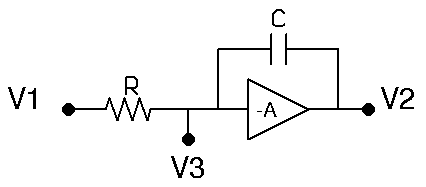
\includegraphics[width=0.4\textwidth]{miller.png}
\end{center}


	\item[(c)] Find the Thevenin resistances $R_{BC}$ and $R_{BE}$ for the following circuits. 

\begin{center}
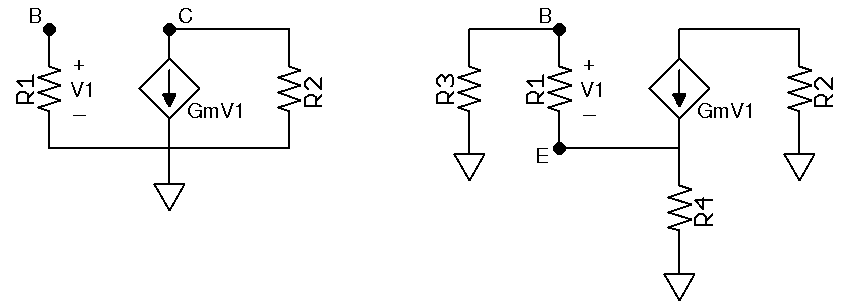
\includegraphics[width=0.8\textwidth]{thevenin.png}
\end{center}


\end{enumerate}
\clearpage


\subsection*{Problem 2: Transistor parameter hunting}
Consider the following circuit, where $V_{be}=-0.6V$, $\beta=200$, and $V_A=80$.
Find $I_S$ for the large signal model and find $g_m$, $r_\pi$, and $r_o$ for the hybrid-pi small-signal model.
Draw the small-signal equivalent circuit.		

\begin{center}
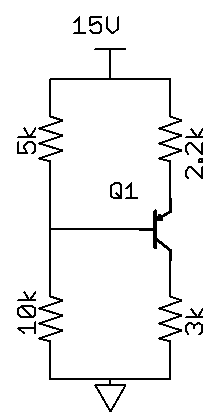
\includegraphics[width=0.2\textwidth]{params.png}
\end{center}

\subsection*{Problem 3: Biasing}
Consider the following circuit, where for\\
Q1: $I_S=10^{-15}A$, $V_A=\infty$, $V_{CE_{sat}}=0.2V$, $\beta=200$,\\
M1: $V_T = 0.6V$, $\mu_nC_{ox}\frac{W}{L}=200\frac{\mu A}{V^2}$, $\lambda=0$
$V_{cc}=5V$,$R_L=30k$,$C_B$ is large. 

\begin{center}
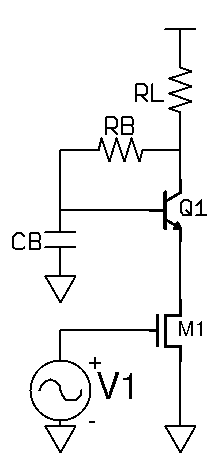
\includegraphics[width=0.2\textwidth]{biasing.png}
\end{center}

\begin{enumerate}
\item[(a)] Determine the DC value of V1 such that $I_{C1}=60\mu A$.
\item[(b)] Find the DC output voltage at the collector of Q1.
\item[(c)] Determine the range of $R_B$ that keeps M1 in saturation and Q1 in the FAR.
\end{enumerate}
\end{document}
